%Note di Ingegneria del Software
%Sommario: Ciclo di Vita, Modelli di ciclo di vita

\cornell{Ciclo di vita}{Solitamente visto come una macchina a stati, in cui si vede la successione di 4 stati:\\
$Concezione \Longrightarrow Sviluppo \Longrightarrow Uso \Longrightarrow Ritiro$\\
Ogni progetto si colloca su un tempo di calendario \underline{finito}, lineare e segmentabile.\\
Ogni segmento temporale è concettualmente detto \textbf{fase}.\\
Il modo in cui mi muovo tra le fasi è deciso dal modello di ciclo di vita.}
\cornell{Code'n'Fix}{È un \textbf{non-modello}, dove prima creo del codice, vedo se funziona ed eventualmente correggo i difetti.\\
Non ha organizzazione preordinata e porta a progetti caotici e difficilmente gestibili.}
\cornell{Modello Sequenziale}{(W. Royce, 1970)\\
Detto anche "modello a cascata".\\
È un modello incentrato sulla ripetibilità del modello stesso e delle proprie fasi (in progetti diversi)\\
È un modello composto da fasi \textbf{rigidamente sequenziali}: \begin{itemize}
\item Nessun Parallelismo
\item Nessuna Sovrapposizione
\item Nessun Ritorno a fasi precedenti
\end{itemize}
È un modello guidato da documentazione, in cui il software arriva solo alla fine. Fa fortissimo uso di pre- e post-condizioni.}
\cornell{Modello Sequenziale di Ciclo di Vita (Secondo lo standard ISO 12207)}{Nello standard, le fasi del ciclo di vista del software sono viste come:\\
$Analisi \Longrightarrow Progettazione \Longrightarrow Realizzazione \Longrightarrow Manutenzione$\\
Dove il software arriva solo nella fase di Realizzazione.\\
Le prime 3 fasi sono dette "Modello sequenziale di Sviluppo"}
\cornell{Caratteristiche del Modello Sequenziale}{\begin{itemize}
\item È un modello iperdisciplinato
\item La quantificabilità (delle misure temporali, di costo, \ldots) dipende fortemente dall'esperienza
\item Sistematico
\item Troppo Rigido
\end{itemize}}
\cornell{Correttivi al Modello Sequenziale}{\begin{description}
\item [Prototipazione] In stile "usa e getta"\\
Aiuta a mitigare il problema della mancanza di codice nelle fasi di Analisi e Progettazione
\item [Cascata con ritorni] Posso permettermi di tornare a fasi precedenti\\
Però produce potenzialmente più incertezze e perdite di tempo (confronta con i modelli iterativi)}
\cornell{Modello Incrementale}{Spesso \textbf{non} conviene integrare tuttle le parti nelle fasi iniziali (cosiddetta "big bang integration"), dato che questo renderebbe arduo il troubleshooting in caso qualcosa non andasse. $\Longrightarrow$ conviene affidarsi ad una integrazione incrementale.\\
Il modello Incrementale prevede molteplici rilasci successivi.\\
Esso inizia analizzando il problema in maniera macroscopica; successivamente si decide quali incrementi fare per soddisfare gli obiettivi più importanti.\\
In questo modo le caratteristiche principali sono pronte prima e quelle minori hanno più tempo per stabilizzarsi ed armonizzarsi con il resto.\\
Successivamente decido come disegnare il modo in cui le componenti andranno ad integrarsi; dopodichè si inizia a sviluppare gli incrementi.\\
Se è possibile è conveniente parallelizzare degli incrementi (per esempio sviluppo di interfaccia e backend di un servizio online), invece di avere fasi strettamente sequenziali.\\
Le fasi di Analisi e Progettazione \underline{non si ripetono}}
\cornell{Modello Incrementale secondo ISO 12207}{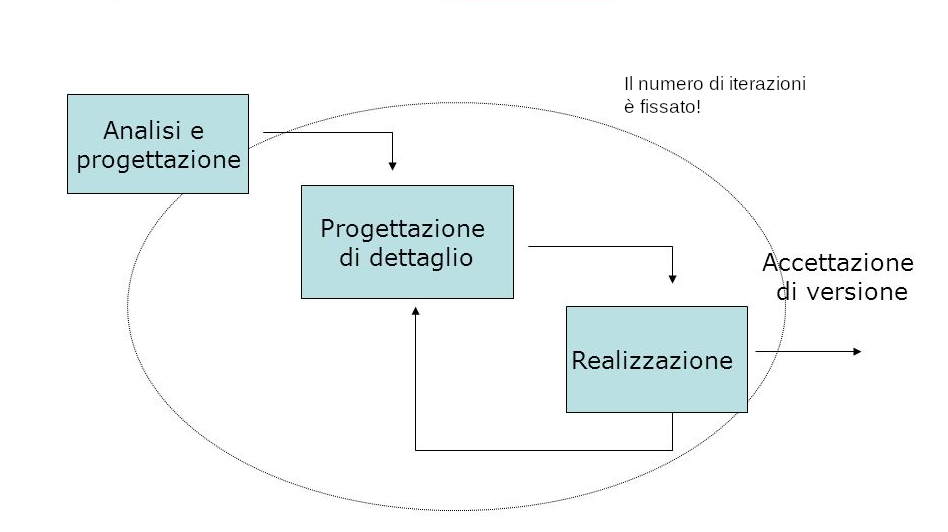
\includegraphics[scale=0.4]{images/3.png}}
\cornell{Modello evolutivo}{Col tempo, i bisogni tendono a flettere, crescere o comunque cambiare con l'uso, quindi non è sempre possibile conoscere l'outline del problema specificatamente\\
Il modello evolutivo è composto da cicli paralleli su più versioni (stable, beta, alpha, \ldots)\\
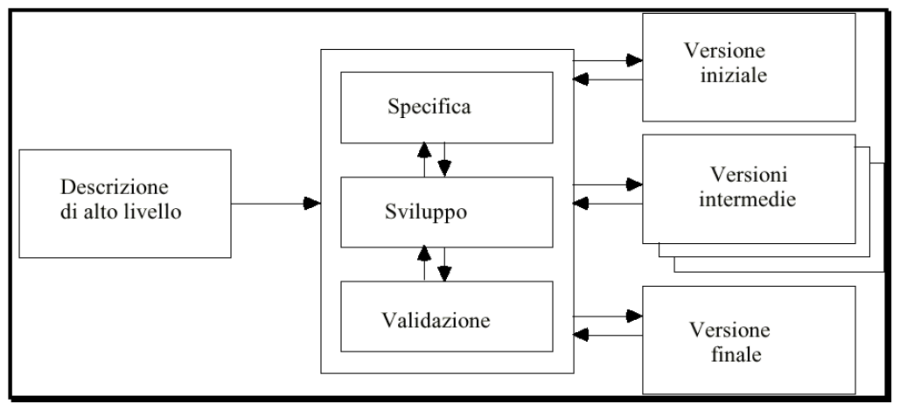
\includegraphics[scale=0.35]{images/4.png}
}
\cornell{Caratteristiche del Modello Evolutivo}{Il modello evolutivo presenta una fortissima sovrapposizione di attività diverse fatte su versioni diverse, un esempio potrebbe essere il ciclo di rilasci di un browser (che qui ho chiamato simpaticamente "WaterDog")\\
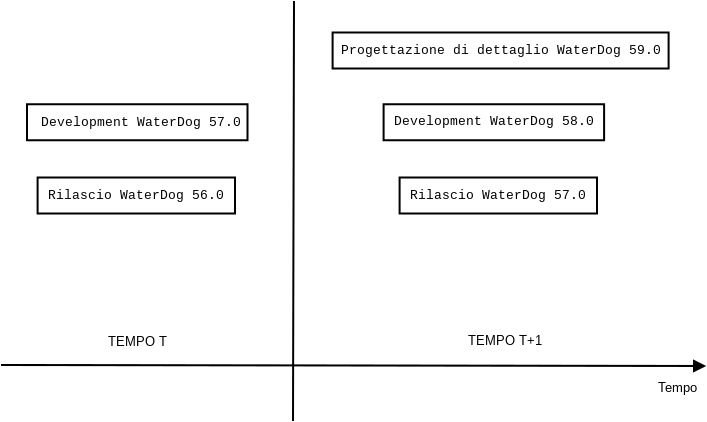
\includegraphics[scale=0.45]{images/5.png}}
\cornell{Modello a componenti}{Basato sul riuso di componenti proprie e di terzi, arrivando persino ad adattare i requisiti in modo da renderli più adatti ad una progettazione a componenti con riuso.\\
È un modello che viene sempre più utilizzato data l'abbondanza di componenti (librerie, per esempio) software.}
\cornell{Modelli Agili: La nascita}{I modelli agili nascono come reazione all'eccessiva rigitidà data dai modelli prevalenti fino alla fine degli anni '90}
\cornell{Modelli Agili: Il Manifesto}{Riferimento: http://agilemanifesto.org/\\
Essenzialmente i modelli agili si basano su questi principi: \begin{itemize}
\item Le regole troppo rigide non fanno bene
\item La documentazione non è tanto importante quanto un software funzionante
\item Invece di negoziare con lo stakeholder, collaboraci
\item Essere pronti a reagire a situazioni in arrivo piuttosto che avere un piano
\end{itemize}}
\cornell{Modelli Agili: Critiche al manifesto}{È necessario rendersi però conto che alcuni punti, così come sono, sono problematici: \begin{itemize}
\item Un software senza documentazione è un costo più che un valore: non basta commentare il codice, è necessario spiegare e motivare certe scelte realizzative.
\item Senza un piano non è possibile valutare i rischi e gli avanzamenti del processo
\item È bene essere in grado di reagire, ma è soprattutto necessario essere consapevoli dei costi e benefici che certi cambiamenti comportano
\end{itemize}}
\cornell{User Story}{I modelli Agili si basano sulle "User Story", dei documenti di descrizione del problema in esame, creati dialogando con l'utente, ascoltandolo, ragionando e proponendo soluzioni e miglioramenti in maniera attiva.\\
Inoltre definisce la strategia per confermare la conformità del software alle richieste del committente.}
\cornell{Esempi di Metodologie Agili}{\begin{description}
\item [Scrum] (Termine del football americano, un'azione apparentemente caotica che in realtà nasconde regole ed organizzazione)
\item [Kanban] (Giapponese, simile al just-in-time)
\item [Scrumban]
\end{description}}
\cornell{Scrum}{Metodologia basata su iterazioni, con le seguenti componenti salienti: \begin{description}
\item [Product Backlog] Essenzialmente una todo list che contiene requisiti e funzionalità del prodotto
\item [Sprint] Si scelgono ed eseguono le fasi ritenute più utili al creare un "incremento utile", dura dalle 2 alle 4 settimane e si ottiene un prodotto potenzialmente vendibile
\item [Sprint Backlog] Essenzialmente una todo list che raccoglie l'insieme di storie per il prossimo sprint
\end{description}}
\cornell{Fasi dello Scrum}{\begin{description}
\item [Sprint Planning] Pianificazione dello sprint
\item [Daily Scrum] Un controllo giornaliero dell'avanzamento, nella forma di un incontro stand-up di circa 15 minuti. $\Longrightarrow$ anche se temporalmente breve è invasivo
\item [Sprint Review] Si controllano i prodotti dello sprint
\item [Sprint Retrospective] Si effettua un controllo qualità sullo sprint
\end{description}}
\cornell{Ciclo di Vita secondo SEMAT}{Se all'interno di ogni componente di progetto SEMAT (opportunity, \ldots) si identificano delle sottofasi, si arriva ad una way of working ripetibile ed adattabile.\\
Da un forte senso di "come facciamo ad avanzare", grazie alle tabelle di progressione.}
